\documentclass[tikz,border=10pt]{standalone}
\begin{document}
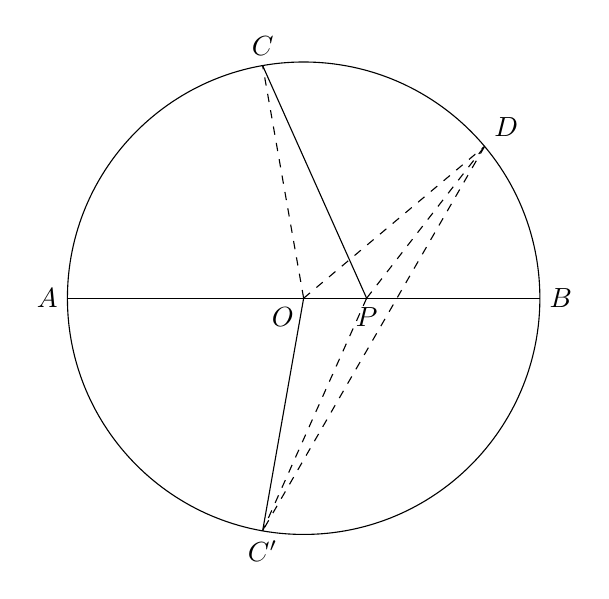
\begin{tikzpicture}
    \coordinate (O) at (0,0);
    \coordinate (A) at (-3,0);
    \coordinate (B) at (3,0);
    \coordinate (P) at (0.8,0);
    \coordinate (C) at (100:3);
    \coordinate (C') at (260:3);
    \coordinate (D) at (40:3);

    \draw (O) circle (3);
    \draw (A) -- (B);
    
    \draw (C) -- (P);
    \draw (O) -- (C');
    
    \draw[dashed] (O) -- (C);
    \draw[dashed] (O) -- (D);
    \draw[dashed] (P) -- (D);
    \draw[dashed] (P) -- (C');
    \draw[dashed] (D) -- (C');
    
    \node[left] at (A) {$A$};
    \node[right] at (B) {$B$};
    \node[below left] at (O) {$O$};
    \node[below] at (P) {$P$};
    \node[above] at (C) {$C$};
    \node[above right] at (D) {$D$};
    \node[below] at (C') {$C'$};
\end{tikzpicture}
\end{document}
